\documentclass[11pt,twocolumn,twoside,lineno]{pnas-new}
% Use the lineno option to display guide line numbers if required.
% Note that the use of elements such as single-column equations
% may affect the guide line number alignment. 

\templatetype{pnasmathematics} % Choose template 
% {pnasresearcharticle} = Template for a two-column research article
% {pnasmathematics} = Template for a one-column mathematics article
% {pnasinvited} = Template for a PNAS invited submission

\usepackage{pdfpages}
\usepackage{booktabs}
\usepackage{tabularx}
\usepackage{graphicx}
\usepackage{subcaption}
\usepackage{multirow}
\usepackage[square]{natbib}
%\usepackage[nohyperlinks, printonlyused]{acronym}

%%enable Paragraphs
\usepackage{pgfgantt}
\usepackage{parskip}
%\usepackage{babel}
%\usepackage{translator}
\usepackage{pdfpages}
 \usepackage{pdflscape}
%\usepackage[hidelinks]{hyperref}

\title{EveryDrum}

% Use letters for affiliations, numbers to show equal authorship (if applicable) and to indicate the corresponding author
\author[1]{Autoren:Tom Ziegler}
\author[1]{Lukas Peschel} 
\author[1]{\\ Betreuer: Dr. Sebastian Merchel}

\affil[1]{Technische Universität Dresden}

\keywords{Drums $|$ Android $|$ Arduino $|$ PureData $|$} 

\begin{abstract}
Wird eine Oberfläche durch einen Anschlag angeregt, so beginnt die Oberfläche zu schwingen. Diese Schwingung kann mittels Beschleunigungssensoren auf der Oberfläche aufgenommen werden.
Diese Schwingung sollen genutzt werden, um verschiedene Anschlagspositionen voneinander unterscheiden zu können.

Verwendet wurde ein Arduino Nano mit einem Kombisensor MPU-6050. 
Die Auswertung der Sensordaten fand auf einem Android-Smartphone statt.
Zur Unterscheidung der Anschlagpositionen wurden aus den aufgenommenen Schwingungen mittels FFT-Analyse die dominantesten Frequenzen ermittelt und der Frequenzabstand zu den erlernten Positionen bestimmt.
Nach erfolgreicher Zuordnung zu einer bekannten Position wurde ein entsprechender Ton abgespielt.

Ziel des Projektes war es, mittels des entstandenen Systems eine beliebige Oberfläche als virtuell erweitertes Percussioninstrument nutzen zu können.


\end{abstract}

\dates{Erstellt am \myformat\today}
%\doi{\url{www.pnas.org/cgi/doi/10.1073/pnas.XXXXXXXXXX}}

\begin{document}

% Optional adjustment to line up main text (after abstract) of first page with line numbers, when using both lineno and twocolumn options.
% You should only change this length when you've finalised the article contents.
\verticaladjustment{-2pt}

\maketitle
\thispagestyle{firststyle}
\ifthenelse{\boolean{shortarticle}}{\ifthenelse{\boolean{singlecolumn}}{\abscontentformatted}{\abscontent}}{}

\section*{Einleitung}
Diese Projektarbeit entstand im Rahmen des Moduls "Virtuelle Realität" im Sommersemester 2018. 
Die Zielstellung war die Entwicklung eines Systems, bestehend aus Hard- und Software, mithilfe dessen eine beliebige Oberfläche als Schlagzeug verwendet werden kann.
Eine angeschlagene Position soll dafür in Echtzeit klassifiziert und einem der vorher erlernten Schlaginstrumente zugeordnet werden.

Die Vergabe der Projektthemen und erste Besprechung dieser erfolgte am 16.04.2018. Am 28.05. erfolgte eine Zwischenpräsentation, im Rahmen dieser die bisherigen Konzepte der verschiedenen Teams gegenseitig vorgestellt und diskutiert wurden. 
Die Abgabe und abschließende Präsentation der Ergebnisse erfolgte am 09.07.2018. 
Der Zeitraum der Bearbeitung erstreckte sich damit über 12 Wochen.

Im Rahmen einer ersten Konzeption wurden folgende Maßgaben für die Umsetzung aufgestellt:
\begin{itemize}
	\item Das entstandene System soll portabel, einfach anzuwenden und wenig spezielle Hardware erfordern
	\item Um ein realistisches Spielgefühl zu erzeugen, soll die maximale Latenz zwischen Anschlag und Abspielen des Sounds 100ms betragen
	\item Das System soll robust funktionieren und dem Anwender ein Feedback über die Zuverlässigkeit der Erkennung liefern, sodass dieser eventuell Verbesserungsmaßnahmen durchführen kann (z.Bsp. Reduzierung von Hintergrundrauschen)
\end{itemize}

Um die Realisierung der Projektidee in diesem Zeitrahmen möglich zu machen, wurden zu Beginn einige Vereinbarungen getroffen:
\begin{itemize}
	\item Als Oberfläche sollen vorerst nur Tische mit Holz- oder Kunststoffplatten verwendet werden
	\item Maximal sollen drei verschiedene Positionen unterschieden werden
	\item Im Sinne einer Prototypentwicklung sollen Funktionalität und Beweis der Konzeptplausibilität höhere Priorität als Benutzerfreundlichkeit haben
    \item In diesem Projekt soll die Eigenschwingung der angeschlagenen Oberfläche zur Auswertung genutzt werden. 
\end{itemize}



\subsection*{Fragestellungen}
\begin{itemize}
	\item Welche Oberflächen eignen sich am besten?
	\item Wie groß muss das Zeitfenster für einen Schlag gewählt werden, um eine robuste Erkennung sowie eine geringe Latenz zu erreichen?
	\item Welche Informationen können aus den Beschleunigungsdaten gewonnen werden, und welche eignen sich zur Echtzeit-Klassifizierung?
	\item Wie kann die Überlagerung zweier Anschläge verhindert/verringert werden?
\end{itemize}
%  \section*{Zetiplan}
 \begin{landscape}
 	
\newgantttimeslotformat{stardate}{
	\def\decomposestardate##1.##2\relax{\def\stardateyear{##1}\def\stardateday{##2}
	}
	
	\decomposestardate#1\relax
	\pgfcalendardatetojulian{
	\stardateyear-01-01}{#2}
	\advance#2 by-1\relax
	\advance#2 by\stardateday\relax
	}
%April
\begin{ganttchart}[hgrid,vgrid,time slot format=stardate, inline,
	milestone inline label node/.append style={left=5mm}]
	{2018.99}{2018.120}
	\gantttitlecalendar{, month=name, day}\\
	\ganttgroup{Einführung}{2018.99}{2018.106}\\
	\ganttbar{Signalerfassung und DrumSounds}{2018.107}{2018.120}
\end{ganttchart}
%Mai
\begin{ganttchart}[hgrid,vgrid,time slot format=stardate, inline,
	milestone inline label node/.append style={left=5mm}]
	{2018.121}{2018.151}
	\gantttitlecalendar{, month=name, week} \\
	\ganttbar{Prototyp Singnaleinbindung}{2018.121}{2018.134}\\
	\ganttbar{Prototyp Testen}{2018.136}{2018.145}\\
	\ganttmilestone{Zwischenpräsentation}{2018.146} \\
	\ganttbar{Verbessern}{2018.147}{2018.151}
	\ganttlink{elem0}{elem1}
	\ganttlink{elem1}{elem2}
	\ganttlink{elem2}{elem3}	
\end{ganttchart}
%Juni - Juli
\begin{ganttchart}[hgrid,vgrid,time slot format=stardate, inline,
	milestone inline label node/.append style={left=5mm}]
	{2018.152}{2018.195}
	\gantttitlecalendar{, month=name, week}\\
	\ganttbar{Erweitern \& verfeinern}{2018.152}{2018.171}\\
	\ganttbar{Testen}{2018.172}{2018.179}\\
	\ganttbar{Präsentation vorbereiten}{2018.175}{2018.182}\\
	\ganttbar{Puffer}{2018.182}{2018.188}\\
	\ganttmilestone{Endpräsentation}{2018.189} 
	\ganttlink{elem0}{elem1}
	\ganttlink{elem1}{elem2}	

	\ganttlink{elem2}{elem3}
	
	\ganttlink{elem3}{elem4}
\end{ganttchart}

\end{landscape}


\section{Konzept}
Ein naiver Ansatz wäre, mehrere Sensoren auf der Oberfläche zu verteilen und eine ein- oder zweidimensionale Lokalisation mittels Bestimmung der Laufzeitunterschiede durchzuführen.
Dies setzt allerdings die Verwendung mindestens zweier (eindimensional, max. 3 Positionen) bzw. dreier (zweidimensional) Sensoren. 
Die Verwendung mehrerer Sensoren bedeutet jedoch auch steigende Anforderungen an die verarbeitende Hardware, höherer Realisierungsaufwand, höhere Anforderungen an den Anwender und nicht zuletzt höheren Hardwareaufwand und -abhängigket, was die Portabilität und Verwendbarbarkeit deutlich einschränkt.

Daher soll lediglich ein Sensor verwendet werden. Dies bedeutet jedoch, dass die Unterscheidung der Anschlagpositionen lediglich anhand der Schwingungscharakteristiken erfolgen muss.

Wird eine Tischplatte an einer Position angeschlagen, führt diese eine Eigenschwingung aus.
Je nach Material, Lagerung, Obejekte auf der Oberfläche, etc... unterscheiden sich verschiedene Tischplatten in ihrer Impulsantwort.
Außerdem unterscheidet sich die ausgeführte Schwingung je nach Position und Art der Erregung: 
Ein Schlag mit den Fingerknochen erzeugt eine andere Schwingung als ein Schlag mit der flachen Hand - dies lässt sich leicht anhand des entstehenden Geräusches verifizieren.
Ebenso erzeugt ein Schlag auf die Tischkante eine andere Schwingung als ein Schlag in die Tischmitte - dies zeigt sich vor allem in unterschiedlichen Nachhallzeiten.

Gewisse charakteristische Eigenschaften sind bauartbedingt durch den Tisch vorgegeben. 
Diese können vom Anwender nicht beeinflusst werden, folglich muss die Software in der Lage sein, diese Unterschiede in der Verarbeitung zu berücksichtigen. 
Trotzdem hat der Anwender gewisse Möglichkeiten, die Schwingung der Tischplatte zu beeinflussen, beispielsweise durch Anbringen von Massen, Dämpfern, etc... 
Dies kann und soll bewusst eingesetzt werden, um die Schwingungscharakteristiken der Anschlagspositionen möglichst unterschiedlich zu gestalten.  

Um eine hohe Flexibilität in der Anwendung zu liefern, soll auf die Verwenung eines PCs/Laptops verzichtet werden. Stattdessen soll die softwareseitige Umsetzung mittels eines Smartphones erfolgen.

Zur Aufnahme der Schwingung wurden verschiedene Möglichkeiten erprobt:
\begin{itemize}
	\item Verwendung eines Piezzosensors
	\item Verwendung des internen Beschleunigungssensors des Smartphones
	\item Verwenung eines Arduino Mikrocontrollers mit Beschleunigungssensoren  
\end{itemize}


\section{Umsetzung}
Für die Umsetzung wurde ein Android-Smartphone, ein Lenovo K6, mit der Android-Version 7.0 verwendet.
Hingegen zu älteren Smartphones, unterstützen neuere den .... Modus, womit die Stromversorgung des Arduinos über USB-Anschluss gewährleistet wird.


\section{Arduino}


\subsection{CH340}

\cite{CH340}
\subsection{ MPU 6050}
\section*{Signalanalyse}
\label{sec:Signalanalyse}
\subsection*{Anschlagserkennung}
Zur Erkennung von von Anschlägen und Abgrenzung von Hintergrundrauschen werden die Messdaten in Echtzeit geprüft. Hierzu werden die jeweils letzten beiden Messwerte miteinander verglichen. Ein Anschlag wird erkannt, wenn der aktuellere Wert den vorherigen Wert um ein bestimmtes Vielfaches der Standartabweichung übersteigt. Der Faktor sollte dabei auf das zu erwartende Rauschen abgestimmt werden - höhere Werte neigen weniger dazu, Ausschläge im Rauschen bzw. unabsichtliche Behrührungen der Oberfläsche als Anschlag zu erkennen, niedrigere Werte erlauben dagegen, auch sanfte Anschläge zu erkennen. In unseren Versuchen hat sich ein Faktor von 6 als stabil erwiesen.

Wurde ein Anschlag erkannt, so beginnt ein Zeitfenster von ca. 500ms, in dem eingehende Messwerte gepuffert werden. Nach Ablauf des Zeitfensters wird dem Programm signalisiert, dass ein Schlag aufgenommen wurde. Zusätzlich werden die Messwerte bis ca. 20ms vor dem erkannten Anschlag in die Zeitreihe aufgenommen.

\subsection*{Analyse der Beschleunigungsdaten}
Die Klassifizierung aufgenommener Schläge erfolgt mittels Auswertung der stärksten Frequenzen. Hierzu werden die Messwerte zunächst einer diskreten Fouriertransformation unterzogen, und die Spektrale Leistungssdichte der Zeitreihe bestimmt.
In der aktuellen Implementierung konnten Abtastraten von ca. 200Hz erreicht werden. Die größte damit detektierbare Frequenz $f_{max}$ liegt somit bei 100Hz.
Für ein Zeitfenster von ca. 500ms ergeben sich 128 Messwerte.
Nach Anwendung der Fouriertransformation erhält man somit 64 diskrete Frequenzgruppen mit einer Trennschärfe von ca. 2Hz.

Aus diesen Daten werden die 4 Frequenzanteile mit der höchsten Amplitude ermittelt zur weiteren Verwendung gespeichert.

\subsection*{Lernphase}
Zum Erlernen einer Schlagposition werden zwölf Schläge aufgezeichnet, wie oben beschrieben analysiert. und anschließend der Durchschnitt der jeweils stärksten Frequenzgruppe, zweitstärksten Frequenzgruppe, usw. ermittelt, wie in Abb. \ref{fig:FFT_Mittelwerte} zu sehen ist. Diese werden als charakteristisches Muster gespeichert.

Tabelle \ref{tab:FFT} zeigt die zwölf Schläge zum Lernen für Hihat und Bass.
Die Schläge wurden auf einer Tischplatte ausgeführt mit unterschiedlicher Position für HiHat und Bass.
Es ist zu erkenne, dass die Unterschiede zwischen den Mittelwerten größer sind, als zwischen den Median-Werte in Abb. \ref{fig:FFT_Median}.

\begin{figure}[H]
	\centering
	\caption{Stärkste Frequenzen}
	\begin{tabular}{l c c c c | l c c c c}
		HiHat &&&& &Bass \\
		\hline
		Frequenz & F1 & F2 & F3 & F4  & & F1 & F2 & F3 & F4\\	
		& 13 & 14 & 15 & 19  &&13& 114& 115& 87\\
		& 30 & 31 & 23 & 24 &&13& 28& 29& 30\\
		& 13& 14& 15& 16 &&35& 36& 23& 24\\
		& 29& 30& 13&36 &&13& 14& 15& 62\\
		& 17& 23&24& 30 	&&15& 16& 42& 43\\
		&13& 24& 25& 47	&&13& 54& 30& 31\\

		&27& 15& 16& 17	&&20& 89& 90& 39\\

		 &17& 18& 30& 31 &&13& 20& 26& 27\\

		&42& 43& 44& 55		&&19& 20& 29& 30\\

		 &25& 33& 34& 35 &&19& 20& 13& 26 \\

		&22& 23& 13& 37		&&13& 14& 15& 16\\

		&31& 32& 14& 15  &&13& 58& 59& 60\\
		\\
		\hline
		Durchschnitt & 23,25&	25	&22,167& 30,167 && 16,583	&40,25&	40,5&	39,583	\\
		Median & 23,5 &	23,5& 19,5	& 30,5 && 13 &	24	& 29	 &30,5 \\		 
		

	\end{tabular}
	\label{tab:FFT}
\end{figure}

\begin{figure}[H]
\centering
\begin{subfigure}{.5\textwidth}
		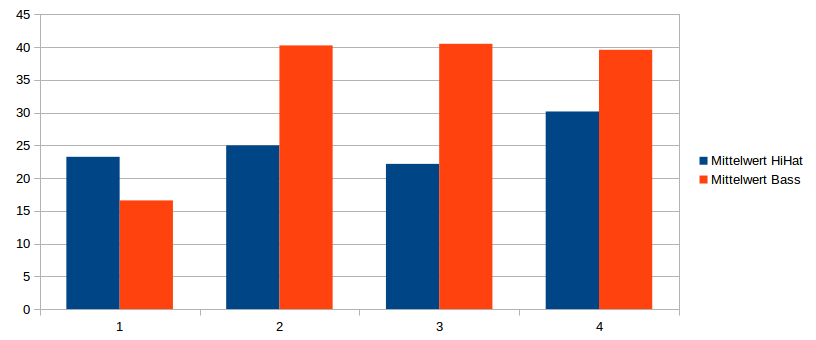
\includegraphics[scale=0.5]{figures/Mittelwert_hihatbass.png}
\end{subfigure}
\caption{Mittelwerte von Hihat und Bass für Frequenzen F1 - F4}
\label{fig:FFT_Mittelwerte}
\end{figure}


\begin{figure}[H]
\centering
\begin{subfigure}{.5\textwidth}
		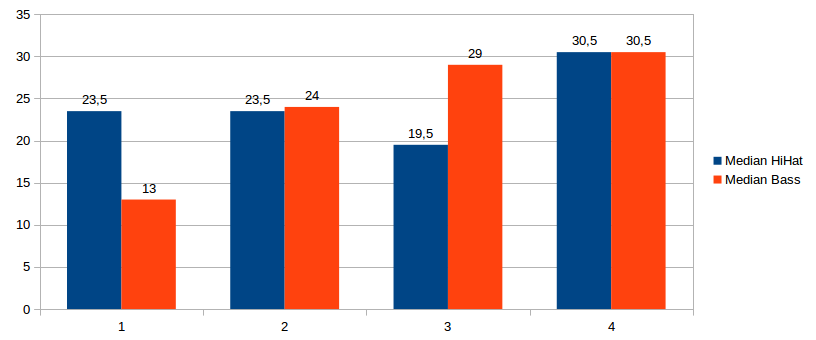
\includegraphics[scale=0.5]{figures/Median_hihatbass.png}
\end{subfigure}
\caption{Median-Werte  von Hihat und Bass für Frequenzen F1 - F4}
\label{fig:FFT_Median}
\end{figure}


\subsection*{Echtzeit-Klassifizierung}
Ist die Echtzeit-Klassifizierung aktiviert, so werden nach erfolgter Anschlagserkennung und Schlagaufzeichnung die Messwerte analysiert und mit denen der gelernten Positionen verglichen. 
Für diesen Vergleich werden die Frequenzabstände der jeweils stärkste Frequenzgruppen, zweitstärksten Frequenzgruppen, usw... ermittelt und die Teilergebnisse zu einer totalen Abweichung aufsummiert.

Nachfolgend ist so eine Klassifizierung mittels der im Abschnitt "Lernphase" eingeführten Beispieldaten dargestellt:


 
Erkennbar hierbei ist, dass in jedem Falle eine Zuordnung erfolgt - auch wenn die Abweichung absurd groß ist. Dies könnte jedoch leicht geändert werden, indem eine maximale Abweichung festgelegt wird und alle berechneten Abweichungen, die diesen Wert übersteigen, als nicht klassifizierbar eingestuft werden. Alternativ könnte, ähnlich zu anderen Clustering-Verfahren, eine Nachbarschaftsbeziehung zur Klassifikation verwendet werden.

\subsection*{Signalaufbereitung/Filterung}

In der aktuellen Implementierung wird keine Filterung der Messdaten vorgenommen. 
Um die Genauigkeit der Frequenzanalyse zu erhöhen, sollten die Messwerte vor Anwendung der FFT mit einem Tiefpassfilter mit der Grenzfrequenz $f_{max}$ gefiltert werden.

Eine Möglichkeit, um Rauschen zu unterdrücken wäre die Nutzung eines Grenzwertes. Auf diese Art können schwache Erschütterungen und leichte Vibrationen unterdrückt werden.
Die Sensordaten könnten weiter geglättet werden durch Verwendung eines Box-Filters (Moving-Average) oder Gauss-Filters.

%Anstelle von timbreID, welches laut Entwickler \cite{timbreID} Cluster benutzt und Merkmale sortiert, haben wir den DBSCAN-Algorithmus getetest.

%Elbatta und Ashour untersuchen verschiedene Clustering Ansätze und stellen in ihrer Arbeit \cite{Elbatta2013ADM} einen verbesserten DBSCAN-Algorithmus vor.
%DBSCAN ist ein  dichtebasierter Cluster-Algorithmus, der als Parameter einen Radius und eine Mindestanzahl an Punkte pro Cluster benötigt.
%Im Gegensatz zu partitionierungsbasierten Cluster-Algorithmen, wie zum Beispiel K-Means, besitzt DBSCAN dne Vorteil, dass es freie Formen von Clustern erkennen kann und sich besonders gut für Daten mit %Rauschen eignet.
%Der Algorithmus startet mit einem zufälligen Punkt.
%Befinden sich die Mindestanzahl an Nachbarpunkten um den gewählten Punkt im gegebenen Radius, wird ein Cluster mit allen gefunden Punkten gebildet.
%Ist die Anzahl Nachbarpunkte kleiner als die Mindestanzahl wird dies als Rauschen markiert.
%Es wird rekursiv mit dem nächsten freien Punkt verfahren, der noch nicht zu einem Cluster gehört und noch nicht bewertet wurde.

%Der DBSCAN-Algorithmus könnte somit verwendet werden, um besondere Merkmale von festzustellen und diese von Rauschen zu unterscheiden.

%Ein Clustering mit DBSCAN zeigte bei uns keine guten Ergebnisse, da wohl die Merkmale

\section{Diskussion}
\subsection{Oberfläche}
\textit{Welche Oberflächen eignen sich am besten?}

Im Laufe des Projektes wurde eine Reihe von Testdurchläufen auf verschiedenen Oberflächen ausgeführt. Dazu wurden 2 Position mit jeweils 10 Schlägen angelernt und anschließend 100 Anschläge druchgeführt. Die Dämpfung erfolgte durch eine flach auf den Tisch gelegte Hand realisiert. Zur Bewertung der Oberfläche wurde die effektive Erkennungsrate herangezogen.

Holztisch, leer | 65%
Holztisch, mit Dämpfern | 68%
Kunststofftisch, leer | 60%
Kunststofftisch mit laufenden PCs | 53%

Erkennbar ist, dass zwischen gedämpfter und ungedämpfert Holztischplatte kaum signifikante Unterschiede bestehen. Die Dämpfung könnte jedoch relevant werden, wenn ein schnelleres Spieltempo angestrebt wird, und Schwingungen aus Anschlägen sich überlagern. In unserem Versuch führten wir den nächsten Anschlag erst aus, wenn die Schwingung der Oberfläche durch den vorherigen Anschlag abgeklungen war.

Weiterhin ist erkennbar, dass die Erkennungsrate bei der Kunststofftischplatte geringer war als bei der Holzplatte.


\subsection{Zeitfenster}
\textit{Wie groß muss das Zeitfenster für einen Schlag gewählt werden, um eine robuste Erkennung sowie eine geringe Latenz zu erreichen?}



\subsection{Analyse}
\textit{Welche Informationen können aus den Beschleunigungsdaten gewonnen werden, und welche eignen sich zur Echtzeit-Klassifizierung?}




% Bibliography
\section*{Literaturnachweis}
\bibliographystyle{alpha}
\bibliography{literature}


\end{document}